\documentclass[twocolumn,9pt]{ltjsarticle}

\usepackage[top=20mm,bottom=20mm,left=25mm,right=25mm,columnsep=10mm]{geometry}
\usepackage[haranoaji,nfssonly]{luatexja-preset}
\usepackage{graphicx}
\usepackage{titlesec}
\usepackage{url}

\usepackage{multirow}    % セル結合用
\usepackage{tabularx}    % 表用&カラムサイズ指定

%% カラムサイズの指定用 %%
\newcolumntype{C}[1]{>{\centering\arraybackslash}p{#1}}
\newcolumntype{L}[1]{>{\raggedright\arraybackslash}p{#1}}
\newcolumntype{R}[1]{>{\raggedleft\arraybackslash}p{#1}}

\title{周期解析によるボットネット検出と対処優先度決定手法の提案}
\author{19FMI29 山下 尚彦 \\ 指導教員: 寺田 真敏}
\date{}

\begin{document}
\maketitle

\section{はじめに}
サイバー攻撃において, ボットウイルスと呼ばれるマルウェアの一種に感染した端末で構成されたネットワーク, ボットネットを利用したものがあり, 過去には数百万台の端末が接続されたボットネットが確認された. ボットネットによる攻撃はその巨大なネットワークを利用した攻撃手法が特徴で, そのひとつに, サーバに対してボットネットに参加する複数の端末から大量のアクセスさせてサーバをダウンさせるDDoS攻撃がある. 実際に, 2016年10月にDNSサービスを提供するアメリカの企業が, IoT機器を標的とするMiraiというボットウイルスによって形成されたボットネットによるDDoS攻撃を受け, 一時的にサービスが停止しDNSを利用していたTwitterやSpotify, PayPalなどの主要サービスにも影響が及び, その被害額1億1000万ドルと推定される事件が起こった. また, スパムメール配信の踏み台や仮想通貨を稼ぐためのマイニング, 広告の自動クリックなどの攻撃者にとって利益となる行為や脆弱なサーバ情報の収集やクレジットカード番号の収集などのスパイウェアとしての活動に利用される. このように, ボットウイルスに感染した端末に対して破壊活動や身代金の要求などを行わずに攻撃者の遠隔操作により秘密裏に攻撃活動を行うためボットの発見は非常に困難になっている. 

攻撃者はボットネットに接続する膨大な数の端末を制御するために, コマンド\&コントロール(C2)サーバと呼ばれる踏み台サーバを利用してボットの更新や攻撃命令などを行う. また, ボットネットに接続する端末に対して定期的に通信を行い, ボットネットの状態を確認する. 

本研究の目的は, ネットワークの通信を収集し周期を分析することで, C2サーバとボットネットの定期的な通信の検出とC2サーバのレスポンスによって対処の優先度を決定することにある. 本稿では, 総務省実証事業「サイバー攻撃解析・防御モデル実践演習の実証実験の請負」で実施され, 研究者コミュニティから提供された組織内ネットワークへの侵害活動を観測したデータセット「動的活動観測2016(BOS\_2016)」\cite{マルウェア対策研42:online}を周期分析した実験の概要と結果, その考察と今後の課題について述べる. 

\section{関連研究}
本章では, 関連研究と本研究との違いを述べる. 

AsSadhanらはC2サーバとボットネット間の周期的な通信を検出する手法を提案した\cite{assadhan2018analysis}. AsSadhanらの研究では, C2サーバとの通信に比較的よく使われる通信プロトコルであるIRC, P2P, HTTPの規定ポート番号の11375, 6667, 80番ポート上の通信を収集し, 周波数解析によって悪意のある通信の検出を試みた. 

実際に大学のネットワークで実験を行った結果, IRCやP2Pによる通信の周期性を検出できたものの, HTTPを使った通信はボット以外のアプリケーションが膨大な通信を行っていたため検出することが困難であった. また, 規定のポートを使用しないボットに関して検出できないという課題があると言及していた. 

本研究では通信の周期性を検出する際に, ポート番号で通信をフィルタリングするのではなく, 送信元と受信先のIPアドレスごとに通信をグループに分けるという点で異なる. 送信元と受信先のIPアドレスでグループに分けることでボット以外のアプリケーションによる通信の影響を受けにくくすることを目的とする. また, 3.1で説明するLomb-Scargleピリオドグラムによって通信の周期分析を行うという点でも異なる. 

\section{提案手法}
本章では, C2サーバとボットネット間の周期的な通信を検出する手法とボットネットの対処優先度を決定する手法について述べる. 

\subsection{周期性のある通信の検出手法}
本節では, 通信観測データの前処理と周期性の検出方法について述べる. 

\subsubsection{解析前処理}
ネットワーク上の通信を観測したデータから周期性の検出に必要な次の5つの情報を抽出する. 

\begin{itemize}
    \item 通信時間のタイムスタンプ
    \item 送信元IPアドレス
    \item 受信先IPアドレス
    \item 通信プロトコル
    \item 通信データの中身
\end{itemize}

通信時間のタイムスタンプと送信元IPアドレス, 受信先IPアドレスは周期性の検出に, 通信プロトコルと通信データの中身は3.2節で説明するボットネットの対処優先度を決定に使用する. 必要な情報の抽出後, 送信元IPアドレスと受信先IPアドレスのペアとなるようにデータをさらに分割する. 

\subsubsection{Lomb-Scargleピリオドグラムによる解析}
Lomb-Scargleピリオドグラムによる周波数解析\cite{vanderplas2018understanding}を用いて通信の周期性を検出する. Lomb-Scargleピリオドグラムは不定間隔, または欠損のある信号であっても周波数解析を行うことができ, 図\ref{fig:lombscargle}のような連続していない正弦波の周期性を推定することができる. 

本研究では, 3.1.1項で得られたデータをLomb-Scargleピリオドグラムで解析し, 周期性のある通信を検出する. 

\begin{figure}[htbp]
    \centering

    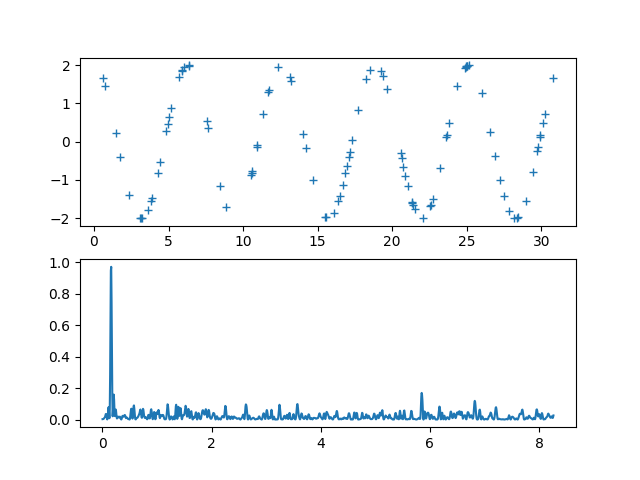
\includegraphics[width=7.5cm]{images/【実験】LombScargleピリオドグラムによるShinoBot通信の解析/lombscargle.png}

    \caption{欠損のある正弦波と解析結果}
    \label{fig:lombscargle}
\end{figure}

\subsubsection{周期性の有無の測定}
周期性の有無は, 信号が周期性のない正規分布であると仮定して, Lomb-Scargleピリオドグラムで信号を解析した結果, ピークがしきい値を超えたかどうか判断する. 図\ref{fig:lombscargle}を例にすると, 図\ref{fig:lombscargle}上部の正弦波が1\%の確率で非周期的な信号であると仮定し, Lomb-Scargleピリオドグラムの解析結果である図\ref{fig:lombscargle}下部のグラフのピークが0.18631798を超えた場合, 99\%周期的である確率が高いと言える. このグラフのピークは0.9993959064009751なので, 図\ref{fig:lombscargle}の正弦波は99\%以上周期的である. 

\subsection{対処優先度の決定手法}
通信プロトコルにHTTPを利用したリクエストは通信先からHTTPレスポンスを受け取る. このHTTPレスポンスには, リクエストが正常に完了したかどうかを示す3桁の数字からなるレスポンスステータスコードが含まれる. ステータスコードは主に200番台, 400番台, 500番台が使われ, 200番台はリクエストが正常に完了したことを表し, 400番台はURLの間違いによってサーバがリソースを発見できなかったことを示す404(Not Found)などのクライアントによるエラー, 500番台はサーバ側で処理できない事態が発生した500(Internal Server Error)などのサーバ側で起きるエラーを示す. 

本研究では, HTTPベースのボットネットがC2サーバと通信して受け取ったステータスコードによってボットネットの対処優先度を決定する. 3.1節で周期性を検出した通信のうち, HTTP通信を行った通信のステータスコードが200番台であれば緊急性のある事案とし, 400番台の場合は, C2サーバは稼働している可能性があるがボットネット側のエラーによってリクエストが正常に完了していないので, 200番台ほどではないが対処する必要がある事案とする. さらに400番台の中でのステータスコードによってエラーの種類がわかるため, 更に細かく優先度を設定できると考えられる. 500番台に関してはC2サーバ側でエラーが発生しているため優先度を低くすることができる. 

\section{実験}
本章では, データセットBOS\_2016の概要と実験に使用したデータ, 条件について述べる. 

\subsection{データセットBOS\_2016概要}
本研究の実験で使用するデータセットBOS\_2016は, 総務省実証事業「サイバー攻撃解析・防御モデル実践演習の実証実験の請負」で実施され, 研究者コミュニティから提供された組織内ネットワークへの侵害活動を動的に観測したデータセットである. マルウェア検体のハッシュ値情報や, 通信観測データ, プロセス観測データの他に, Windowsのイベントログやファイアウォールのログがデータセットとして提供されている. 

データセットには, マルウェアの動作が確認されC2サーバと正常に通信が発生して攻撃の観測ができた事例(Case e04)やC2サーバへのSYNパケットのみ送信した事例(Case e12, e20), C2サーバとの通信が確認されなかった事例(Case e70, e435), また, 動作が確認されなかった事例(Case e43)の観測データやログなどが記録されている(表\ref{tab:bos2016}). 

\begin{table}[htbp]
    \centering
    \caption{BOS\_2016の検体の挙動と通信について}

    \begin{tabular}{C{2cm}L{1.5cm}L{2.5cm}}
        %% カラム名 %%
        \hline
        Case & 挙動 & 通信 \\
        \hline \hline
        %% データ %%
        e04 & 動作 & 攻撃活動を観測 \\ \hline
        e12\par e20 & 動作 & C2サーバとの通信が成立しない(403, 404, 503) \\ \hline
        e43 & 実行不可 & 通信発生せず \\ \hline
        e70\par e435 & 動作 & C2サーバへSYNパケットのみ送信 \\
        \hline
    \end{tabular}

    \label{tab:bos2016}
\end{table}

\subsection{実験に使用したデータ}
本研究では, ネットワークから周期性のある通信の検出を検出するためにデータセットの通信観測データを使用する. 動的活動観測環境でマルウェアの検体を実行した機器のうち, e04はマルウェアが動作し実際に攻撃を観測したため, 通信観測データが提供されていなかった. よって, 実験ではe12, e20, e43, e70, e435の通信観測データと観測環境内で観測された通常の通信を含む全ての通信観測データを用いる. 

\subsection{実験条件}
本研究では, 通信観測ータを1日ごとに分割してLomb-Scargleピリオドグラムで解析する. また, Lomb-Scargleピリオドグラムで解析した結果, 周期的である確率が90\%以上である信号を周期性のある通信とする. 

\section{結果}
本章では, 4.2節で説明した通信観測データの周期分析実験の結果について述べる. なお, 本稿ではマルウェア検体が動作しC2サーバとのTCPコネクションを確立したが, HTTPのステータスコードが403(Forbidden),404(Not Found), 503(Service Unavailable)などでC2サーバとの通信が成立しなかったe12とe20の解析結果のみ記述する. 

表\ref{tab:e12}と表\ref{tab:e20}は, e12とe20の通信観測データを1日ごとに解析し, 送信元IP数(SRC), 送信元と受信先IPペア数(PAIR), 周期的である確率が99.9\%以上ある通信を行ったIPアドレスのペア数をまとめた表である. また, 表\ref{tab:e12-e20_ip}は99.9\%以上周期的な通信を示したペアの受信先IPアドレスの結果である. 

\begin{table}[htbp]
    \centering
    \caption{Case e12の実験結果}

    \begin{tabular}{c||lll}
        %% カラム名 %%
        \hline
        DATE & SRC & PAIR & 99.9\% \\
        \hline \hline
        %% データ %%
        20160212  & 21 & 42 & 9 \\
        20160213  & 5  & 8  & 0 \\
        20160215  & 8  & 14 & 7 \\
        20160216  & 4  & 6  & 0 \\
        \hline
    \end{tabular}

    \label{tab:e12}
\end{table}

\begin{table}[htbp]
    \centering
    \caption{Case e20の実験結果}

    \begin{tabular}{c||lll}
        %% カラム名 %%
        \hline
        DATE & SRC & PAIR & 99.9\% \\
        \hline \hline
        %% データ %%
        20160215  & 14 & 27 & 3 \\
        20160216  & 5  & 8  & 1 \\
        20160217  & 5  & 8  & 1 \\
        20160218  & 8  & 15 & 7 \\
        \hline
    \end{tabular}

    \label{tab:e20}
\end{table}

\begin{table}[htbp]
    \centering
    \caption{e12とe20で周期的な通信を示した受信先IPアドレス}

    \begin{tabular}{|c||c|c|}
        \hline
        CASE & DATE & IP ADDRESS \\
        \hline \hline

        e12 & 20160212 & \begin{tabular}{c}
                            213.165.83.176 \\
                            23.32.241.24   \\
                            50.56.81.119   \\
                            52.76.86.155
                         \end{tabular} \\ \cline{2-3}
            & 20160215 & \begin{tabular}{c}
                            104.76.4.147   \\
                            23.59.139.27   \\
                            23.59.160.60   \\
                            61.213.168.19
                         \end{tabular} \\ \hline

        e20 & 20160215 & \begin{tabular}{c}
                            10.32.1.160    \\
                            13.107.4.50    \\
                            216.58.221.163
                         \end{tabular} \\ \cline{2-3}
            & 20160216 & 104.118.6.83 \\ \cline{2-3}
            & 20160218 & \begin{tabular}{c}
                            10.32.1.160    \\
                            199.36.102.106 \\
                            74.113.237.189
                         \end{tabular} \\ \hline
    \end{tabular}
    
    \label{tab:e12-e20_ip}
\end{table}

\section{考察}
本章では, 本研究の実験結果を寺田らがデータセットBOS\_2016について報告した内容\cite{weko_175829_1}を踏まえて考察する. 

寺田らの報告によると, e12やe20のようにマルウェアがC2サーバとのTCPコネクションを確立できた場合, C2サーバにTCP SYNパケットを送信する頻度が低いため通信からC2サーバを特定することは困難であるとしているが, 本研究の実験からe12がC2サーバと行った周期的な通信を特定することができた. また, e20に関してはe20からC2サーバに対するHTTPリクエストの周期性を特定することができなかったが, C2サーバからのHTTPレスポンスの周期性を検出できた. よって, 通信の周期性を検出することで, ボットネットとC2サーバの通信を検出する手法は有効であると考えられる. 

\section{おわりに}
本稿では, データセットBOS\_2016の通信観測データからボットネットがC2サーバと行う周期的な通信の検出手法の実験とその結果について述べた. 

実験の結果, C2サーバとの通信を検出することができ, Lomb-Scargleピリオドグラムによる周期分析は有効であったが, 周期的な通信を行う通常の通信を一定数検出したため, より精度を高めることが必要であると考えられる. 

今後は, 検出精度の向上とC2サーバのHTTPレスポンスステータスコードによる対処優先度を決定するために, C2サーバの状態によってどのようなレスポンスを行うかや危険度の設定方法の調査を行う予定である. 

\bibliographystyle{junsrt}
\bibliography{DB}
\end{document}